
\section{Organisation moderner RISC- und CISC-Prozessoren}

\subsection{Kurze Widerholung RISC und CISC Prinzipien}
\subsubsection{Mikroprogrammierung in CISC-Architekturen}
\begin{itemize}
	\item
		Makrobefehl bildet einstieg in Mikroprogramm

		\begin{figure}[hpbt]
			\centering
			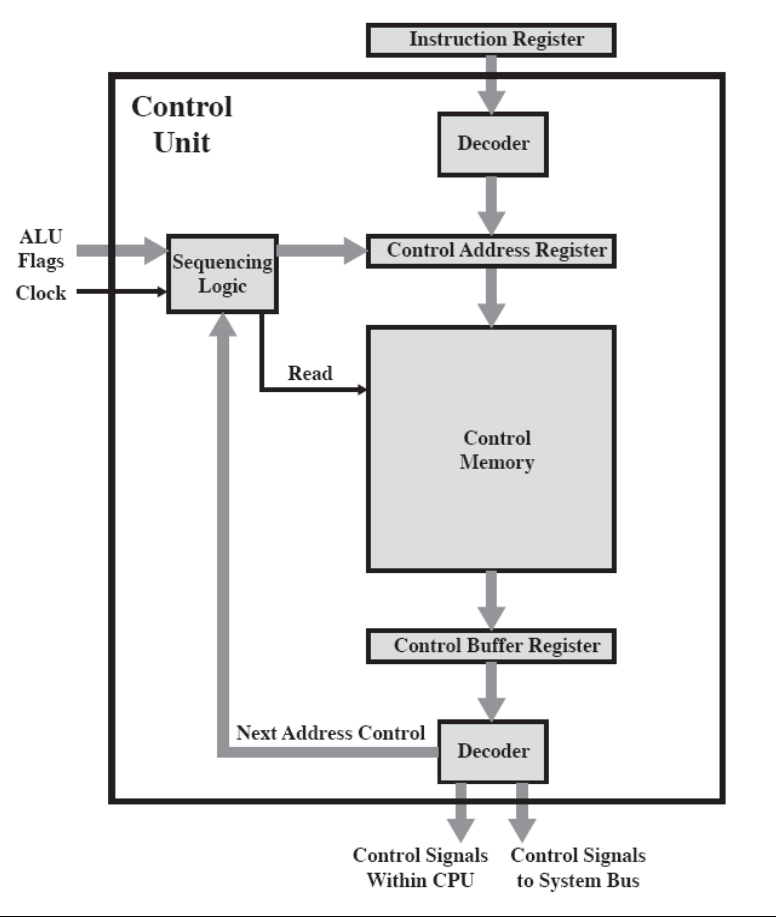
\includegraphics[width=0.5\textwidth]{img/leitwerk_mikro.png}
			\caption{Darstellung der Funktion eines mikroprogrammierten Leitwerks}
			\label{fig:mikroprog}
		\end{figure}
		\item
			Erklärung zu \autoref{fig:mikroprog}:
			\begin{itemize}
				\item
					CAR -- Control Address Register: enthält Adresse der nächsten Instruktion (1. Mikrobefehl des auszuführenden Mikroprogramms)
				\item
					CBR -- Control Buffer Register: nimmt Eintrag aus Mikroprogrammspeicher (CM) auf
				\item
					Sequencing Logic: entscheidet welche Adresse aus CM als nächstes ausgelesen wird:
					\begin{itemize}
						\item
							ALU flags (bedingter Sprung)
						\item
							Nächste Adresse: aus Adressteil des im CBR stehenden Mikrobefehls oder Inhalt CAR oder sequenzielles Fortschalten der letzten Adresse

					\end{itemize}
			\end{itemize}
		\item
			Control Memory besteht aus Sammlung von Mikroprogrammen (für fetch, für indirekte Adressierung, für Interrupts, für opcodes (AND, ADD, \dots)
		\item
			Vorteile Mikropogrammierung: 
			\begin{itemize}
				\item
					CM veränderbar $\Rightarrow$ hohe flexibilität
				\item
					Befehlskompabilität
				\item
					Andere Befehle emulieren
				\item
					Theoretisch Befehlsübersetzung mit Software $\Rightarrow$ virtuelle Maschinen
			\end{itemize}
\end{itemize}

\subsubsection{Pipelining in RISC-Architekturen}
\begin{itemize}
	\item
		Eigenschaften von RISC
		\begin{itemize}
			\item
				Prozessoren der vierten Generation
			\item
				Ziel: elementare und kleine Maschinenbefehlssätze $\Rightarrow$ Operanden und opcode holen während eines Grundtaktes ausführbar
			\item
				Addressberechnungen durch explizite Befehle, keine komplexen Adressierungsarten
			\item
				Operanden in Registern gegeben (load-store-architektur) und große universelle Registersätze
			\item
				festverdrahtete Leitwerke -- kein Mikroprogramm -- Befehl wird direkt in binäres Steuersignal dekodiert
			\item
				konsequentes Pipelining
				\begin{itemize}
					\item
						Execute aller Befehle (außer load/store) innerhalb eines Taktes ausführbar
					\item
						Wegen numerischen float Operationen nicht mehr konsequent durchzuhalten
					\item
						ab Pentium Pro wird komplexer Maschinenbefehl intern in Folge einfachere RISC Befehle zerlegt
				\end{itemize}
			\item
				Zusammenspiel von optimierenden Compiler und RISC Prozessor Arch um pipelining effizient zu nutzen

		\end{itemize}
	\item
		Durchsatz bei Pipelining im Idealfall auf $n$-fache bei $n$ Teilschritten
	\item
		Welche Leistungssteigerung möglich? 
		\begin{itemize}
			\item
				jede pipeline stufe verursacht Zusatz-Aufwand für Datenbewegung $\Rightarrow$ kritisch bei vielen Unterbrechungen im synchronen, sequentiellen Ablauf
			\item
				Mehr Steuerlogik für Register- und Speicher-Abhängigkeiten mit mehr Stufen
			\item
				Pipelinezeit durch langsamste Stufe festgesetzt
			\item
				Zykluszeit $\tau$ einer Pipeline (bestimmt Takt)
				$$
				\tau = \max_i(\tau_i) + d, \qquad d = \text{Zeitverzögerung durch Zwischenspeicherung}$$

			\item
				Erreichbarer Speed-Up $S_k$

		\end{itemize}
	\item
		Preis für Leistungssteigerung
		\begin{itemize}
			\item
				Anstieg HW-Kosten
			\item
				Anstieg Verzögerung
			\item
				Anstieg leerer Pipeline-Zyklen bei Verzweigungen
		\end{itemize}
	\item
		Heute mindestens ein Dutzen Stufen (Intel P4e: 32 Stufen)
	\item
		Weitere Entwicklung: Superskalare Recheneinheiten
		\begin{itemize}
			\item
				Erfordert mehrere Rechenwerke, heute Stand der Technik
			\item
				Gleichzeitige Anwendungen von Ops auf einzelne Komponenten eines Vektors $\Rightarrow$ superskalar
			\item
				Benötigt Befehlsgruppierer
			\item
				Umordnung sequentieller Befehle zur Laufzeit für parallel $\Rightarrow$ dynamische Parallelisierung
			\item
				Allgemeines Prinzip von superskalaren Rechnern: keine direkte Parallelität sondern Herausziehen von Parallelität aus sequentiellem Befehlsstrom
			\item
				Problem: Datenabhängigkeiten/Datenhazards

				Wenn Ergebnis von vorheriger Operation als Operand benötigt wird
			\item
				Lösung: Scoreboard und Tomasolu (siehe \ref{scoreboard} und \ref{tomasolu})
			\item
				Problem: Sprünge -- nächster Befehl in Pipeline ist gar nicht der richtige
				
		\end{itemize}

\end{itemize}

\subsection{Hazards beim Pipelining}
\begin{itemize}
	\item
		Struktur, Kontroll, Daten - Hazards
		\begin{figure}[hpbt]
			\centering
			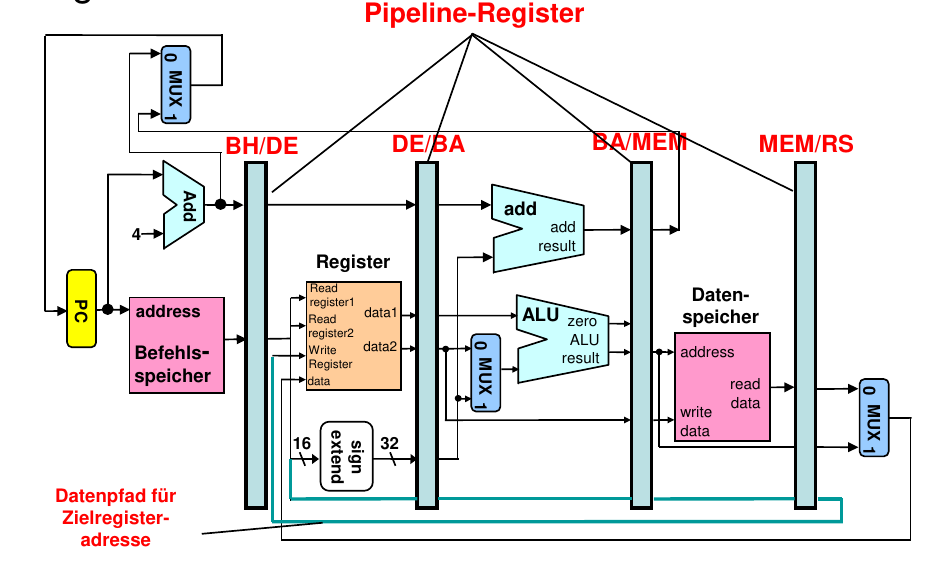
\includegraphics[width=1.1\textwidth]{img/datenpfad.png}
			\caption{Datenpfad zur Darstellung von Hazards}
			\label{fig:hazards}
		\end{figure}
	\item
		5 Phasen: Befehl Holen (BH), Befehl Dekodieren (DE),  Befehl ausführen (BA), Speicherzugriff (MEM), zurückschreiben (RS)
\end{itemize}


\subsubsection{Struktur Hazards}
\begin{itemize}
	\item
		Beispiel für strukturhazard: nur ein Speicherport, Befehl 1 ist Load, macht Speicherzugriff in Takt 4, Befehl 3 will da aber Befehl holen $\lightning$
	\item
		Falls kein Multi-Port Speicher: Pipeline anhalten, stalls einfügen
	\item
		In DE-Phase werden Schreibzugriffe protokolliert und bei erwartenden Konflikten stalls eingefügt

\end{itemize}
\subsubsection{Steuerungshazards}
\begin{itemize}
	\item
		Gegenmaßnahme: Zumeist spekulative Befehlsausführung bzw. Sprungvorhersage
	\item
		Sprungvorhersage:
		\begin{itemize}
			\item
				Statisch: taken, not taken ($>50\%$ richtig), by opcode ($>75\%$ richtig)
			\item
				Dynamisch:
				\begin{itemize}
					\item
						Branch loop buffer (wahrscheinlich aufeinanderfolgende Befehle speichern)

						Nicht nur 1 Befehl speichern sondern Folge von Befehlen. beschleunigt Befehlshohlphase im Falle Entscheidung Sprung

						FIFO organisiert
					\item
						Branch prediction buffer (vorhersage durch Sprung Vorhersagepuffer)

						Speichert zu jedem Verzweigungsbefehl die Historie (mit 1-$n$ bits)
					\item
						Branch history table / branch target buffer (Vorhersage durch Sprung Zielpuffer)
						
						Nachteil des branch prediction buffers: Verzweigungsadresse nicht sofort verfügbar, falls auf Verzweigung entschieden wird

						Deswegen: Erweiterung zum branch target buffer, speichter letzten $n$ Sprungbefehle, assoziativer Zugriff

						Zusätzliche Informationen zum Verwzweigungsziel: Verzweigungsziel, evt. gleich Befehle am Verzweigungsziel speichern, ist aber noch aufwendiger
						\begin{figure}[hpbt]
							\centering
							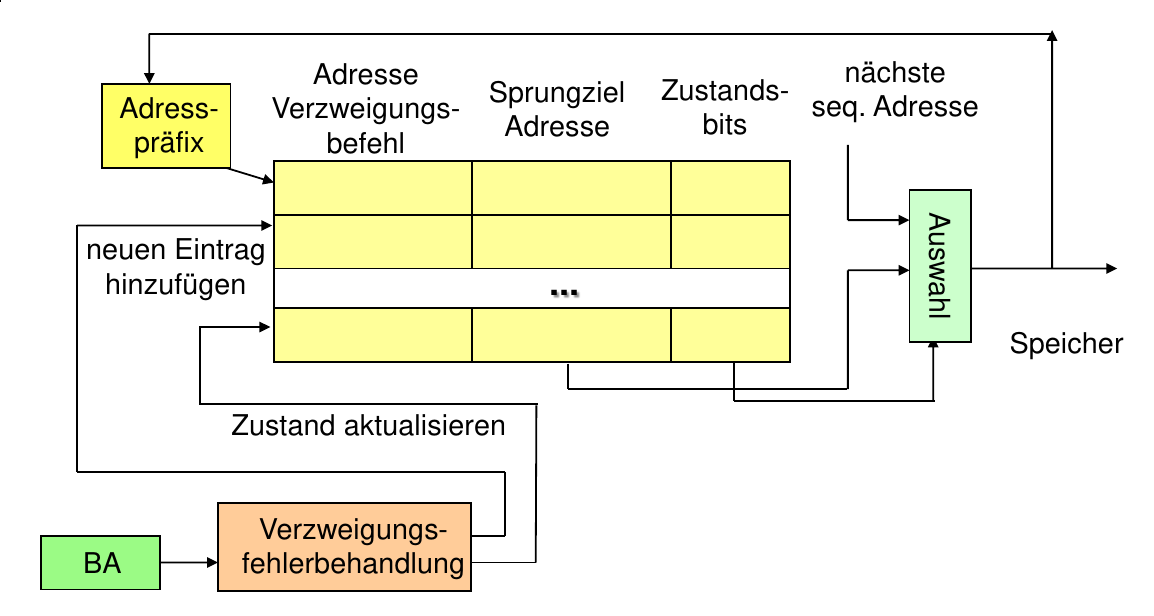
\includegraphics[width=0.9\textwidth]{img/branchtargetbuffer.png}
							\caption{Funktionsweise und Aufbau des branch target buffers}
							\label{fig:btb}
						\end{figure}
				\end{itemize}
			\item
				Statisch:
				\begin{itemize}
					\item
						Delayed branch: Auswertung des Sprungbefehles vorziehen, evt. dann Sprung ohne Pipeline zu stören ausführen

						Evt. hier TODO
					\item
						Andere statische Gegenmaßnahmen, falls zu vergleichende Register bekannt: zusätzliche Berechnungs-HW, z.B. zusätzliches XOR, berechnung während DE

						Durch zusätzlichen Addierer auch Ziel Wert schon aus Konstante im Befehl und aktuellem BZ berechnen
				\end{itemize}

		\end{itemize}
	\item
		Oder: mehrfache Befehlsausführung: beide Zweige ausführen, nur einen behalten. Was wenn weitere Verzweigungen auftauchen? Struktur-Hazards?
\end{itemize}

\subsubsection{Daten-Hazards}
\begin{itemize}
	\item
		3 Typen von Daten hazards: RAW, WAR, WAW
	\item
		RAW: Instr2 liest einen Operanden den Instr1 noch nicht geschrieben hat.
	\item
		WAR: Instr2 schreibt einen Operanden bevor diesen die früher gestartete Operation Instr1 gelesen hat (überholt Instr1 quasi). Kann in einfachen Pipelines in denen lesen vor schreiben stattfindet nicht passieren
	\item
		WAW: Instr2 schreibt Operanden der von früher gestarteter Operation Instr1 überschrieben wird

\end{itemize}

\subsection{Hazard-Auflösung}
\begin{itemize}
	\item
		Gegenmaßnahme:
		\begin{itemize}
			\item
				Forwarding (berechnete Ergebnisse nicht nur an REgister sondern auch an ALU Eingänge zurück) macht alles viel komplizierter
			\item
				Umordnung Befehlsabfolge in SW (Code Scheduling, wird in EPIC Architekturen gemacht)
			\item
				in HW durch dynamic scheduling (vereinfacht Compilerbau, Code bleibt portierbar, zur Compilezeit unbekannte Abhängigkeiten werden berücksichtigt

				Abweichen vom ursprünglichen Ablaufsplan durch out of order execution oder out of order commits/completion
		\end{itemize}
\end{itemize}
\subsubsection{Scoreboard}
\label{scoreboard}
\begin{itemize}
	\item
		Erlaubt instruktionsausführung ohne Rücksicht auf Reihenfolge im Code
	\item
		Vorraussetzung: keine strukturellen und keine RAW hazards
	\item
		zweiteilige DE/ID Stufe
		\begin{enumerate}
			\item
				Issue stage: befehl bekanntmachen, dekodieren, auf strukturelle Hazards prüfen
			\item
				Read operands: warten bis keine Datenhazards mehr vorhanden, dann lesen der Operanden
		\end{enumerate}
	\item
		Idee stammt vom Großrechner CDC66000 -- mitte der 60er Jahre!
	\item
		Out-of-order-commit kann zu WAR und WAW Hazards führen
		\begin{itemize}
			\item
				Lösung für WAR: entweder Operationen jeweils mit Kopien ihrer Operanden verwalten (tomasulo) oder Register erst schreiben, wenn Operanden gelesen wurden
			\item
				Lösung für WAW: Hazard erkennen und warten bis Konflikt bereinigt ist
		\end{itemize}
	\item
		4 Stufen der Scoreboard verarbeitung:
		\begin{enumerate}
			\item
				Decode 1 und auf strukturelle Hazards checken: checken ob Funktionseinheit frei, keine andere Instruktionen mit selbem Zielregister anhängig (WAW$\lightning$)

				Falls gegeben, OP an Funktionseinheit senden und Scoreboard aktualisieren, falls nicht stalls für aktuelle Instruktionen erzeugen und keine weiteren Instruktionen aktivieren (in order issue)
				
			\item
				Operand lesen: Warten bis keine Datenhazards, dann Lesen der betroffenen Register (decode 2)
				\begin{itemize}
					\item
						Quelloperand ist nutzbar wenn früher aktivierte Instruktion ihn schreibt und die Instruktion endet oder wenn Operandenregister gar nicht erst benutzt wird
					\item
						Ist Quelloperand nutzbar, aktiviert Scoreboard funktionseinheit zum Lesen und Starten der Verarbeitung
					\item
						RAW wird dynamisch aufgelöst, Operationen werden out-of-order executed und gleichzeitig an Funktionseinheiten geschickt
				\end{itemize}
			\item
				OP ausführen. Bei Multizyklus OP wird Scoreboard benachrichtigt, wenn OP beendet
			\item
				Rückschreiben der Ergebnisse. Überprüfen ob WAR vorliegen kann, wenn ja stalls einfügen bis Hazard aufgelöst

		\end{enumerate}
						\begin{figure}[hpbt]
							\centering
							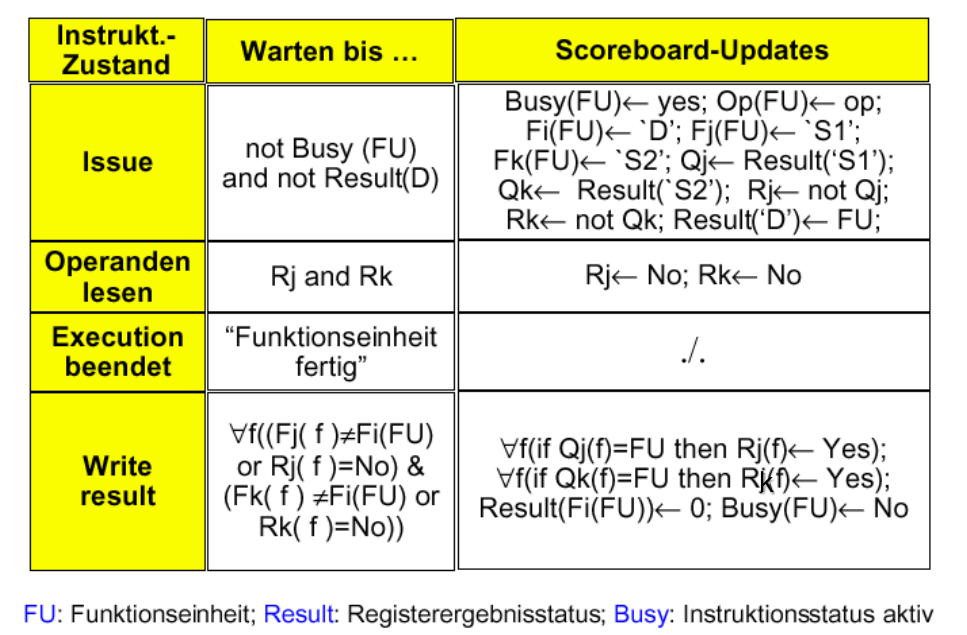
\includegraphics[width=0.7\textwidth]{img/scoreboard.png}
							\caption{Scoreboard Steuerungsalgorithmus, S1 op S2 $\rightarrow$ D, $F_i$ Zielregister, $F_j,F_k$ Quellregister, $Q_j,Q_k$ Funktionseinheiten die Quellregisterdaten erzeugen, $R_j,R_k$, Flags die anzeigen ob $F_j$ oder $F_k$ nutzbar sind}
							\label{fig:scoreboard}
						\end{figure}
\end{itemize}
\subsubsection{Tomasolu}
\label{tomasolu}

\begin{itemize}
	\item
		KOmbiniert Register-Umbenennung mit Scoreboard um WAW und WAR Hazards zu vermeiden
	\item
		Führt Reservierungseinheiten ein: Steuer und Zwischenspeicher
	\item
		Registerreferenzen in Instruktionen werden durch konkrete Datenwerte oder Zeiger auf ReservierungsStationen ersetzt
	\item
		Resultate von Berechnungen werden nicht über Register sondern über gemeinsamen Datenbus an alle Funktionseinheiten verteilt
	\item
		Load Store sind auch Funktionseinheiten mit Reservierungsstationen
	\item
		Registerergebnisstatus zeigt für jedes Register an, welche FU darauf schreibt
		\begin{figure}[hpbt]
			\centering
			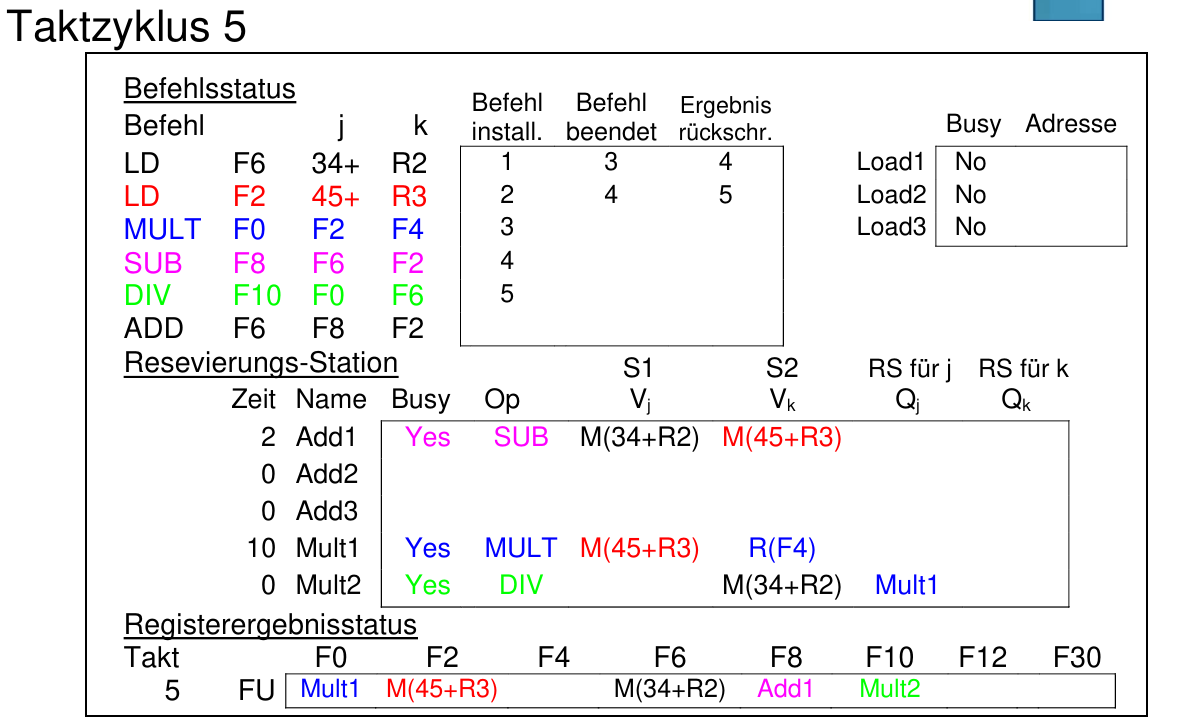
\includegraphics[width=0.9\textwidth]{img/tomasulo.png}
			\caption{}
			\label{fig:tomasulo}
		\end{figure}

	\item
		Vorteil Tomasulo: Vermeidung von wAW und WAR Hazards durch Register Umbenennung/Kopieren, Forwarding
	\item
		Nachteil Tomasulo: mehr HW aufwand, komplexere Kontrolllogik, assoziative Speicherung

\end{itemize}
\subsubsection{Erweiterung um Reorder-Buffer}
\begin{itemize}
	\item
		Ergebnisse kommen in reihenfolge des Codes in den Reorder Buffer
	\item
		Zwischenpuffer um Ergebnisse als in-order-commit zurückzuschreiben
	\item
		Bei Exceptions klar klar, welche Instruktionen abgeschlossen sein dürfen
\end{itemize}
\subsection{Cache Architekturen}
\begin{itemize}
	\item
		Mehrstufige Speicherhierarchie schafft Abhilfe für langsamen und begrenzten Speicher
	\item
		Register \ra{} L$_{1,2,3,4}$-Cache \ra{} Hauptspeicher \ra{} Festplattencache \ra{} Festplatte
	\item
		Cache speicher Blöcke, bestehend aus mehreren Worten \ra{} zeitliche und räumliche Lokalität von Daten Grundlage von effizienten Caches
\end{itemize}
\subsubsection{Cache-Organisation}
\begin{itemize}
	\item
		HIerarchie, Cache Typen und Anordnung:
		\begin{itemize}
			\item
				L1 / Primär
				\begin{itemize}
					\item
						Bestandteil jedes Mikroprozessors
					\item
						Split-Cache: getrennte Speicherung von Daten und Befehlen
					\item
						\SI{32}{kB} bei Intel Sandy-Bridge -- Sky-Lake
					\item
						Kurze Blöcke: \SIrange{32}{64}{B}
				\end{itemize}
			\item
				L2 / Sekundär
				\begin{itemize}
					\item
						Unified-Cache: Daten und Befehle zusammen
					\item
						Größe: \SI{256}{KB} -- \SI{2}{MB}
					\item
						\idr\ gleiche Blockgröße wie L1
				\end{itemize}
			\item
				Mittlerweile Tertiär / L3 Caches: bei sandy bridge core i7 (\SI{1}{MB}), Sandy Bridge Xeon (1--\SI{20}{MB})

		\end{itemize}
	\item
		Platzierung/Identifikation
		\begin{itemize}
			\item
				Cache Organisation legt 2 Dinge fest:
				\begin{itemize}
					\item
						Platzierungsproblem: welcher Hauptspeicherblock in welchen Cacheblock
					\item
						Identifikationsproblem: gewünschtes Datum im Cache wiederfinden
					\item
						3 Typen: direct, voll assoziativ, n-fach assoziativ
				\end{itemize}
		\end{itemize}
	\item
		Direct mapping
		\begin{itemize}
			\item
				Mit $\mod$ wird jeder HS Adresse $B$ ein Block $m$ von insgesamt $N$ Cache-Zeilen zugewiesen: $m = B \mod N$

				\texttt{0x000001, 0xffff01, 0xacab01}  kommen in gleichen Cacheblock
		\end{itemize}
	\item
		Voll assoziativ: beliebige Abbildung
	\item
		n-Fach assoziativ:
		\begin{itemize}
			\item
				Cache Blöcke werden in $s$ Mengen mit jeweils $n$ Blöcken unterteilt: $s = \frac{N}n$
			\item
				HS Block kommt innerhalb der Menge an belibigen Platz
			\item
				allgemeiner Fall, für $n=N$ vollassoziativ, für $n=1$ direkt
			\item
				Abbildung HS Block \ra\ Cache-Block ist surjektiv (HS Block kann in mehreren Cacheblöcken gespeichert werden)

				\Ra\ zusätzlich zu Datenwerten Kennung notwendig, die HS Block safe identifiziert: Tag
			\item
				HS Adresse in zwei Teile mit $w+s$ Bits aufteilen
			\item
				Niederwertigsten $w$ bits identifizieren eindeutig Wort
			\item
				Höchstwertigen $s$ bits spezifizieren Speicherblock
			\item
				Höchstwertigen Bits nochmals aufteilen: 
				\begin{itemize}
					\item
						Feld mit $r$ (Index-)Bits = Adresse der Cache Zeile
					\item
						Feld mit $s-r$, das dem Tag (ermöglicht eindeutige Identifizierung des HS Blocks im Cache) entspricht
				\end{itemize}
			\item
				Beispiel: 24 bit HS Adresse \todo{Übungen zu Tags im Cache etc.\ machen}
				\begin{itemize}
					\item
						\SI{16}{MB} großer Hauptspeicher
					\item
						24 Bit Adresse ($2^{24}$ = \SI{16}{MB}
					\item
						Cache ist \SI{64}{KB} groß
					\item
						Cache-Zeile, bzw.\ Hauptspeicher-Block \SI{4}{Bytes}
					\item
						$w = \SI2{bit}$, Identifier für Dateneinheit im Block (wegen $4=2^2$ Blockgröße)
					\item
						\SI{22}{bit} bleiben als identifier für HS Block übrig. Davon
						\begin{itemize}
							\item
								$r=\SI{14}{bit}$ für $16 = 2^{14}$ Cachezeilen Einträge
							\item
								8 Bit langes Tag ($=22-14$)
						\end{itemize}

				\end{itemize}
			\item
				Falls Programm 2 HS Blöcke addressiert, die auf selbe Cachezeile abgebildet werden, sind Cache Fehlzugriffe häufig \Ra{} Folgen durch Victim Cache abfangen
			\item
				Victim Cache: Aus Cache verdrängter Eintrag wandert in Victim-Cache: meist zwischen L1 und nächster Stufe angeordnet, geringe Größe (4--16 Zeilen), vollständig assoziativ
		\end{itemize}
	\item
		Vollassoziativer Cache
		\begin{itemize}
			\item
				Kein Index, Speicheradresse nur Tag und Wort
			\item
				Tag einer jeden Cachezeile muss auf Übereinstimmung untersucht werden \ra{} teuer!
		\end{itemize}
\end{itemize}
\subsubsection{Cache-Ersetzungsstrategien}
\begin{itemize}
	\item
		Wann und wie wird Hauptspeicher aktualisiert?
		\begin{itemize}
			\item
				Write through: jede Änderung sofort in übergeordneten Speicher. Immer konsistent, aber aufwändig. L1/L2 arbeitet nach diesem Prinzip
			\item
				Write back: Aktualisierung erst bei VErdrängung, Ausgabeoperation oder Zugriff eines anderen Prozessors. Dirty Bit um Rückschreiben nicht modifizierter Blöcke zu vermeiden.

				Letzte Hierarchiestufe arbeitet nach diesem Prinzip
			\item
				Kombinieren mit Write allocate / write-non-allocate (wasauchimmer)
		\end{itemize}
	\item
		Welche Zeile wird ersetzt?
		\begin{itemize}
			\item
				LRU (alterungsinformation in Cache Verwaltungsbits)
			\item
				LFU (Ersetzen der am wenigsten benutzten Zeile)
			\item
				FIFO (durch Ringpuffer realisierbar)
			\item
				zufällig (pseudo-random)
		\end{itemize}
	\item
\end{itemize}
\subsubsection{Cache-Bewertung}
\begin{itemize}
	\item
		3 Arten von Fehlzugriffen: 3 Cs
		\begin{itemize}
			\item
				Compulsory: erster Zugriff
			\item
				Capacity: Cache einfach zu klein um alle Blöcke die aktuell benötigt werden zu halten
			\item
				Conflict: Adresskonflikt
		\end{itemize}
	\item
		Je größer Cache desto unnötiger hoher Assoziativitätsgrad
	\item
		8-fach assoziativer Cache ist aus praktischer Sicht (miss rate) genauso effektiv  wie ein voll-assoziativer
	\item
		2:1-Cache-Regel: Miss Rate eines Direct-Mapped Cache der Größe $n \approx $ Miss-Rate eines 2-Weg assoziativen Cache der Größe $\frac{n}2$
	\item
		Übergang von 1-fach zu 2-fach assoziativität erhöht Taktzykluszeit um 10\% bei externen, um 2\% bei internen Caches \ra{} vernachlässigbar für interne Caches
	\item
		Leistungsbetrachtungen
		\begin{itemize}
			\item
				mittlere effektive Speicherzugriffszeit $T_a = T_h + m\cdot T_m$

				$m$ miss rate, $T_m$ miss penalty (nachladezeit), $T_h$ zugrifffszeit (hit time)
			\item
				Reduzierung von $m$:
				\begin{itemize}
					\item
						durch erhöhung der Kapazität oder des Grades an Assoziativität: erhöht Zugriffszeit $T_h$
					\item
						Durch Erhöhung der Blockgröße: erhöht Nachladezeit $T_m$
					\item
						Bei Direktabbildenden Caches: Victim Cache
					\item
						pre-fetching
				\end{itemize}
			\item
				Reduzierung von $T_h$:
				\begin{itemize}
					\item
						$T_h$ PrimärCache: entscheidend für Prozessortaktrate
					\item
						$T_h$ SekundärCache: entscheidend für Wartezyklen
					\item
						$T_h$ reduzieren durch kleinen, oder einfacher Organisationsstruktur -- aber nachteilig bzgl.\ Fehlrate $m$
				\end{itemize}
			\item
				Reduzierung $T_m$
				\begin{itemize}
					\item
						Durch SekundärCache: $T_m$ wird selbst zu $T_a = T_h + \dots$
					\item
						Einführung nicht-blockierender Caches: nachladen und Zugriff bei Misses gleichzeitig möglich, mehrere ausstehende Speicherzugriffe gleichzeitig
					\item
						$T_m$ maßgeblich durch Prozessor/Systembus bestimmt
				\end{itemize}
		\end{itemize}
	\item
		Höhere Assoziativitätsgrad \Ra{} höhere Taktzeiten
	\item
		Je größer Block Block, \Ra{} Fehlrate steigt wieder leicht an, vor allem bei kleiner Gesamtgröße
	\item
		Je größer Blocksize, desto länger dauert $T_m$
	\item
		Cache-Bewertung Zusammenfassung:
		\begin{itemize}
			\item
				N-Fach assoziativer Cache erfordert $n$-Komparatoren
			\item
				direkt abbildender Cache nur 1 Komparator, da Cache-Zeile eindeutig fest steht. Braucht jedoch häufiges Umladen \Ra{} wirksamkeit sinkt
			\item
				bei assoziativen Caches W'keit für Conflicts geringer
			\item
				Am besten bei voll-assoziativem Cache, aber langsam und teuer
			\item
				In heutigen Prozessoren: Grad 2, 4, oder 8 bzw.\ 16. Wirtschaftlicher und Technischer Kompromiss
		\end{itemize}
\end{itemize}
\subsubsection{Ausnutzen von Cache-Effekten}
\begin{itemize}
	\item
		Daten
		\begin{itemize}
			\item
				Array-Merging (verbesserung räumliche Lokalität durch Verbundarray statt zwei Arraya)
			\item
				Schleifenvertauschung (Vertauschung von Schleifenverschachtelungen um Datenzugriff in Speicherordnung zu erzwingen)
			\item
				Schleifenfusion (Zusammenfassen zweier Schleifen mit selber Durchlaufcharakteristik und überlappenden Variablen
			\item
				Blocking (Verbesserung zeitlicher Lokalität durch Zusammenfassen von Daten zu kompakten Blöcken anstatt zeilen- und spaltenweise durchlaufen)

		\end{itemize}
	\item
		Array-Merging, Schleifenvertauschen, Schleifenfusion, Cache-Blocking (grob), Funktionsweise, Einfluss auf zeitliche/örtliche Lokalität? (162--169)
\end{itemize}

\subsubsection{Cache-Kohärenz}
\subsection{Optimale Pipelinetiefe}
